\chapter{数据集}
对模型的空间推理能力进行充分评估,高质量的数据集必不可少。本章将详细介绍如何构造用于空间推理SRASP数据集,并对数据集的质量进行测试。

\section{设计目标}
尽管CLEVR数据集至今仍被广泛应用于多模态模型的空间推理能力研究,但其存在着一些较为明显的问题,其中比较凸出的是,CLEVR数据集中的场景是完全可观察的,模型可以直接从图像中获取所有必要信息。现实世界中,有很多信息并不能直接从图像中获取。人类基于图像对问题进行回答时,除了直接从图像中观察到的信息,往往也需要使用已经积累的先验知识。本文在此对空间推理的问题进行如下定义:如果回答该问题所需要的全部知识均已包含在图像中,即回答问题不需要使用先验知识,那么称该问题为完全可观察问题。同理,如果图像中并不包括回答该问题所需的全部知识,也即回答该问题需要使用已经积累的先验知识,那么称该问题为不完全可观察问题。

为了解决这一问题,本章基于CLEVR数据集,构建一个名为SRASP的数据集。该数据集的主要设计目标聚焦于以下几个方面:
\begin{enumerate}[label=(\arabic*),itemsep=0pt,parsep=0pt]
\item 考察模型对不完全可观察问题的解答能力。通过引入部分可观察性,模拟现实世界中物体被遮挡或隐藏的场景,要求模型在不完整的视觉信息下进行推理,考察模型真正解决问题的能力。
\item 考察模型对推理密集型问题的解答能力。现实世界的同一场景中,往往存在多个物体,物体之间的关系多样,解决空间推理问题需要多个步骤,逐步解决。通过增大解决问题所需的推理跳数,可以确保模型无法通过简单的模式匹配或者直接观察得出答案,进而真正考察模型的思考和推理能力。
\item 考察模型的知识整合能力。正如在数学证明中定理之间相互印证产生新的定理一样,回答问题所需要的知识,往往也是需要将现有知识进行结合产生新知识,才能最终解决问题。在SRASP数据集中,为每个场景提供一组逻辑约束作为背景知识,模型需将这些先验知识与观察到的视觉信息相结合,以生成正确的答案。
\end{enumerate}

\section{物体基本属性与约束}
与CLEVR数据集中的几何体一样,SRASP数据集的图像中的每个物体,均有形状、尺寸、材质、颜色四种属性。每种属性的可能取值如下:
\begin{enumerate}[label=(\arabic*),itemsep=0pt,parsep=0pt]
    \item 形状:圆锥体、球体、圆柱体和立方体。
    \item 尺寸:小、中、大。
    \item 材质:橡胶、金属。
    \item 颜色:红色、蓝色、绿色、黄色、灰色、棕色、紫色、青色。
\end{enumerate}

除上述四种基本属性之外,图像中的物体也有“所在区域”这一属性,可取值为0、1、2、3。由于所有图像都被划分成
4个区域,故图像中物体也会处在某一个区域之中。为了研究问题方便,本文规定每个物体只能在图像的一个区域中,不能
同时跨多个区域。物体包含这一属性能够为指定约束提供便利。在本数据集中,约束是一组规则的集合,对场景生成
与推理而言密不可分,其主要作用包括:(1)限制物体的属性组合,如对颜色、形状等进行限制;
(2)定义物体之间的关联关系;(3)支持对遮挡物体的推理,当物体被遮挡时,通过约束可以缩小潜在答案的范围。

基于对物体的应用范围,约束可以划分为以下三类:
\begin{enumerate}[itemsep=0pt,parsep=0pt]
    \item 区域约束:仅作用于特定区域的局部规则。例如,“区域1中所有物体形状必须为立方体”。
    \item 跨区域约束:涉及多个区域的全局规则。例如,“区域1和区域2中同颜色物体的总数不超过2个”。
    \item 全局约束:适用于整个场景的通用规则。例如,“所有物体必须属于至少一个区域”或“不允许存在完全相同的两个物体属性组合”。
\end{enumerate}

约束通过使用ASP来进行表示。例如:
\begin{lstlisting}
    :- object(X), at(X, 0), not hasProperty(X, shape, cube), not hasProperty(X, shape, cylinder).
\end{lstlisting}
表示如果X在区域0,那么它的形状必须是立方体或圆柱体。

\section{构造流程}
在确定图像中物体的基本属性之后,本文进一步确定了构建数据集的如下步骤流程:
\begin{enumerate}[itemsep=0pt,parsep=0pt]
\item 生成一组由约束定义的环境,记作$Environment_i$。
\item 生成一个完整的场景图$Complete_i$。该场景图完全符合上一步生成的环境$Environment_i$的要求。
\item 通过从完整场景图$Complete_i$中删除一个物体$Obj_i$,来生成一个部分场景图$Partial_i$。
\item 生成一个对于部分场景图$Partial_i$,对物体$Obj_i$的有关情况进行提问的问题$Q_i$。
\end{enumerate}

\section{环境表示定义}
SRASP中的环境是由一组约束来定义的。与场景相比,环境是一个更抽象一层的概念。针对某个特定的环境,
可以生成以其为模板的场景。可以理解为,环境是场景的抽象,场景是环境的实例。
每个约束决定了特定环境下物体的属性限制。本文首先设计了10个约束模板,所有模板使用ASP来进行表示。
每个环境最多通过20个不同的实例化后的模板来创建,也即每个环境中最多包含20个不同的约束。
部分约束模板的ASP编码表示以及对应表示含义见表\ref{tab:asp_templates}。最终,一共生成了50个
环境,数据集中的每个场景都是由其中一个环境进行实例化后生成的。环境的具体示例见附录\ref{appendix:environment}。

\begin{table}[!h]
    \centering
    \renewcommand{\arraystretch}{1.0}
    \begin{tabular}{|p{3cm}|p{12cm}|}
        \hline
        \textbf{模板} & \textbf{描述} \\
        \hline
        \textbf{模板1(取值约束)} & 
        \texttt{:- object(X), at(X, R), not hasProperty(X, P1, V1).} \\ 
        & 解释: 对区域R中的所有物体,它们P1属性的取值均为V1。 \\ 
        & 具体实现: :- object(X), at(X, 0), not hasProperty(X, color, red). \\
        \hline
        
        \textbf{模板2(否定约束)} & 
        \texttt{:- object(X), at(X, R), hasProperty(X, P1, V1).} \\ 
        & 解释:对区域R中的所有物体,它们的P1属性的取值,均不能为V1。 \\ 
        & 具体实现::- object(X), at(X, 0), hasProperty(X, material, metal). \\
        \hline
        
        \textbf{模板3(恰有N个约束)} & 
        \texttt{:- \#count\{X: hasProperty(X, P1, V1), object(X), at(X, R)\} != N.} \\ 
        & \textbf{解释}:在区域R中,恰好有N个物体的P1属性的取值为V1。 \\ 
        & 具体实现::- \#count\{X: hasProperty(X, size, small), object(X), at(X, R')\} != 2. \\
        \hline
        
        \textbf{模板4(至少有N个约束)} & 
        \texttt{:- \#count\{X1, X2: sameProperty(X1, X2, P1), object(X1), object(X2), at(X1, R1), at(X2, R2)\} < N.} \\ 
        & 解释:在区域R1和区域R2中,至少有N对物体,它们的P1属性的取值都是V1。 \\ 
        & 具体实现::- \#count\{X1, X2: sameProperty(X1, X2, shape), object(X1), object(X2), at(X1, 1), at(X2, 2)\} < 1. \\
        \hline
        
        \textbf{模板5(或约束)} & 
        \texttt{:- object(X), at(X, R), not hasProperty(X, P1, V1), not hasProperty(X, P1, V2).} \\ 
        & 解释:区域 R中的所有对象都具有属性 P1 的 V1 值或属性 P2 的 V2 值。 \\ 
        & 具体实现::- object(X), at(X, 1), not hasProperty(X, color, yellow), not hasProperty(X, color, blue). \\
        \hline
    \end{tabular}
    \caption{部分约束模板示例}
    \label{tab:asp_templates}
\end{table}
\section{场景表示定义}
场景是环境的实例。
SRASP数据集以场景图的形式表示场景,其节点表示使用其属性进行注释的对象,边表示对象之间的空间关系(前、后、左、右)。
在SRASP中,除了场景图表示之外,也用ASP对场景进行表示。
以下展示图\ref{}中部分场景的ASP​表示:
\begin{lstlisting}
%场景中的物体
object(0). object(1). object(2). object(3).

%物体的属性
at(0, 2).
hasProperty(0, color, green).
hasProperty(0, size, large).
hasProperty(0, material, rubber).
hasProperty(0, shape, cylinder).
....

%物体间的空间关系
front(1, 0). right(1, 0). ...
\end{lstlisting}

其中涉及到的谓词的功能如下:谓词\texttt{object}用于定义不同的物体(所有物体的名称用0,1等数字来表示)。
谓词\texttt{hasProperty(Object, Attribute, Value)}用于将对象的名为Attribute的属性的值设置为Value。
对象之间的空间关系用谓词\texttt{left}、\texttt{right}、\texttt{front}、\texttt{behind}来表示,例如
\texttt{left(A, B)}表示B位于A的左侧。
\section{图像生成}
图像生成基于前文中定义的场景图。场景图是一种对场景中物体、属性及其空间关系的结构化描述,而环境则由一系列约束条件所决定,
这些约束可能包括空间分布、物体间的相对关系以及特定属性的限制。
因此,场景图的生成问题可以归结为一个复杂的推理问题:在给定的环境约束(基于ASP的规则)以及场景中预期的物体数量$n$这两个前提下,完成以下任务:
\begin{enumerate}[itemsep=0pt,parsep=0pt]
\item \textbf{区域划分}:将每个物体合理分配到预定义的四个区域之一,确保满足诸如区域容纳量、相邻关系及物体间可能的干扰等约束;
\item \textbf{属性赋值}:为每个物体赋予颜色、尺寸、形状和材质等属性,其取值必须与环境中规定的约束条件一致。例如,某些区域可能只允许出现特定颜色或尺寸范围的物体;
\item \textbf{关系一致性}:在属性分配过程中,还需要确保各物体之间的关系(如邻近、对称或排斥关系)符合逻辑规则,从而保证场景图整体的合理性和一致性。
\end{enumerate}

为了解决上述推理问题,本文采用了ASP的方法。ASP作为一种声明性逻辑编程范式,特别适合解决复杂约束和组合优化问题。
在本系统中,ASP 求解器的工作流程主要包括以下几个步骤:
\begin{enumerate}[itemsep=0pt,parsep=0pt]
\item \textbf{约束建模}:将场景的环境约束以及物体属性赋值规则形式化为 ASP 规则。此步骤需要充分利用逻辑公式来描述物体的空间位置、属性取值范围以及各类关系约束;
\item \textbf{回答集计算}:在输入了物体数量$n$和所有相关约束之后,ASP 求解器会计算出满足所有约束条件的解集。每一个答案集代表一种物体属性及区域分配的合理配置,即一种可能的场景图;
\item \textbf{解集筛选与随机采样}:由于满足所有约束的配置方案可能数量巨大,为了使后续图像生成过程具有一定的随机性与代表性,系统从所有可能的解集中随机采样一百万个场景图。这一随机采样策略既保证了生成场景的多样性,也为后续的图像生成提供了充分的候选数据。
\end{enumerate}

在获得充分的场景图后,系统利用 Blender3 进行图像渲染。
Blender3 是一款高效且功能丰富的三维渲染软件,它能够基于场景图的结构信息生成逼真的图像。
渲染过程包括以下几个关键步骤:(1)场景搭建,根据场景图中各物体的位置信息及属性参数,在 Blender3 中自动搭建三维场景;
(2)光照与材质设置,对各物体的材质、光照、纹理等进行设置,确保渲染出的图像在视觉上具有真实感;(3)
图像生成,利用 Blender3 的渲染引擎,将搭建好的场景生成最终图像。

图\ref{pipeline_for_generating_environment}直观展示了从环境约束到场景图构建,再到图像生成的整个流水线过程,为后续工作的深入探讨提供了坚实的理论与实践基础。
\begin{figure}
    \centering
    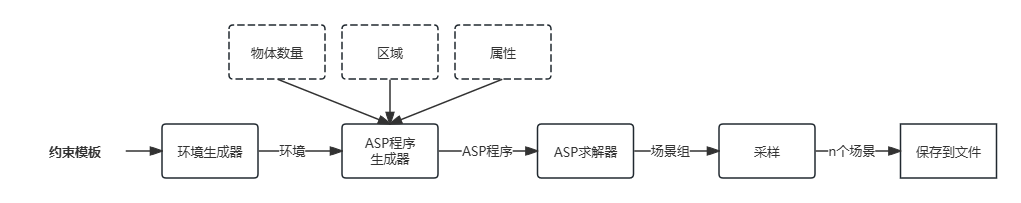
\includegraphics[width=\textwidth]{pipeline_for_generating_environment.png}
    \caption{生成环境以及该环境中的完整场景的流水线}
    \label{pipeline_for_generating_environment}
\end{figure}
\section{问题表示定义}
在SRASP数据集中,每个问题均围绕部分场景中缺失物体的四个关键属性之一:颜色、大小、形状和材质。
问题的设计目标在于通过推理补全场景信息,从而考察系统在不完整场景下对物体属性关系的理解能力。
为此,本文将自然语言描述的问题转化为基于ASP的形式化表示,
使得问题的求解过程可以通过逻辑推理得到明确答案。

数据集中的每个问题最初以自然语言的形式提出,例如:“与中等大小的红色物体的材质相同的,另一个圆柱体的颜色是什么?”
为了使问题具有可操作性,本文设计了对应的ASP编码,如下所示:
\begin{lstlisting}
    query(Q) :- hasProperty(X, color, Q),
    hasProperty(X, shape, cylinder),

    hasProperty(Y, size, medium),
    hasProperty(Y, color, red),
    same_material(Y, X),
    X != Y.
\end{lstlisting}
在该编码中,\texttt{query(Q)}表示需要推导出满足条件的物体X的颜色Q。
此外,通过多个\texttt{hasProperty}和\texttt{same\_material}条件,明确限定了参与推理的物体之间的属性关系,并利用 X != Y 排除自反情况。
这种表示方式不仅使问题的语义精确、结构清晰,而且便于通过 ASP 求解器进行自动求解,从而为数据集中的问题构建提供统一、标准的表达形式。

在问题生成过程中,必须对每个问题的答案范围进行严格控制。对于涉及属性$A$(其中
$A \in \{ color, size, material, shape\}$)的问题,其可能的解集$S$的大小满足$1 \leq |S| \leq |A|$。
其中,$|A|$表示属性$A$所有可能取值的数目。例如,对于尺寸属性,若其可能的取值集合
$\{ large, medium, small\}$,则$|size| = 3$。

如果某个问题生成的解集数量恰好为$|A|$,例如问题答案为“尺寸可以为 large、medium 或 small”,则该问题在特定场景下并未起到区分或推断作用,因此被判定为无效。这一设计思路确保了数据集中每个问题在解答上都具有针对性和挑战性,从而避免生成普遍适用的、无区分价值的答案。
\section{问题生成}
在SRASP数据集中,每个问题均围绕部分场景中缺失物体的某一关键属性展开,如颜色、大小、形状或材质。
为此,本文设计了一套模板,用以指导自然语言问题的生成。以下为问题模板样例:
\begin{lstlisting}
What shape is the < Z2 > (size) < C2 > (color) < M2 > (material) [that is] 
< R > (relation) the < Z > (size) < C > (color) < M > (material) < S > (shape) ?
\end{lstlisting}
其中,<Z2>、<C2>、<M2> 表示待查询对象的已知属性(例如尺寸、颜色、材质),由随机策略从完整场景图中选取;
<R> 为空间关系(如left、right、front、behind),其取值既满足随机性,又依赖于完整场景中物体间的真实空间分布;
<Z>、<C>、<M>、<S> 则代表参考对象的属性,通过对完整场景图中与查询对象具有特定空间关系的候选对象进行筛选而确定。
这种模板化设计不仅使自然语言问题的结构化描述成为可能,而且便于后续转换为ASP的形式化表示,从而实现问题求解的自动化。

问题模板的实例化过程基于与图像对应的完整场景图。具体步骤包括:
\begin{enumerate}[itemsep=0pt,parsep=0pt]
\item 场景图构建与部分场景生成。利用完整场景图构建方法,将真实场景中的物体、属性以及空间关系进行抽象建模;从完整场景中随机移除一个物体,以构造部分场景图,此移除的对象即为“查询对象”,其缺失的属性将作为问题求解目标。
\item 已知属性的随机选取。对于查询对象,模板中的已知属性(例如<Z2>、<C2>、<M2>)由随机采样策略确定,确保不同问题之间在属性分布上具有较好的随机性和代表性;同时,选取的属性应满足数据集整体的“问题类型平衡”要求,避免某一属性出现频率过高或过低。
\item 空间关系的确定。对于模板中表示空间关系的部分(<R>),取值虽然随机,但参考对象的选择依赖于完整场景图中的物体空间布局。具体而言,从与查询对象存在 <R> 关系的物体中进行候选对象的筛选,从而确保问题中提及的空间关系具有实际语义意义。
\end{enumerate}

为了使问题具有可操作性和求解性,所有生成的问题均转化为ASP形式。转换过程中包括以下步骤:
\begin{enumerate}
\item 规则构建。将自然语言问题中的各项约束(属性约束、空间关系约束、对象排他性约束等)以ASP规则的形式表达;
\item 约束整合。同时将部分场景图与环境约束作为求解器的输入,确保问题求解过程在完整逻辑下进行;
\item 解集判定。由ASP求解器计算出问题的所有可能解。针对每个属性$A \in \{ color, size, material, shape\}$
,若生成的解集$S$满足$1 \leq |S| \leq |A|$,则问题被认为具有合理的答案区分性;若解集规模等于$|A|$
说明答案涵盖了属性的全部取值,缺乏针对性,此时问题将被判定为无效并从数据集中剔除。
\end{enumerate}

图\ref{pipeline_for_generating_partial}展示了从完整场景图构建、部分场景生成、问题模板实例化、ASP表示转换,到最终问题求解的流水线过程。
该流程通过随机采样,使生成的问题在属性组合和空间关系上呈现多样性;通过对解集规模的判定机制,
有效过滤掉普遍适用或无区分意义的问题,确保每个问题都能够准确反映场景中物体属性的关系;
使用模板化设计和ASP表示为后续数据集扩充与新问题类型的加入提供了灵活性和统一标准。
\begin{figure}
    \centering
    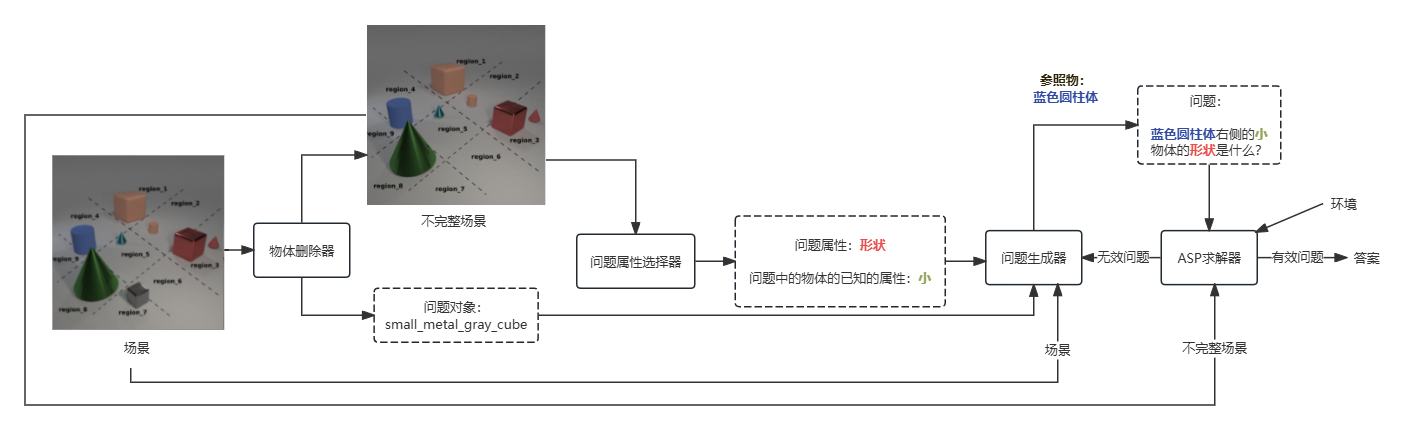
\includegraphics[width=\textwidth]{pipeline_for_generating_partial.png}
    \caption{生成部分场景和问题,并进行标记的流程}
    \label{pipeline_for_generating_partial}
\end{figure}
\section{数据集分析}
\subsection{统计分析}
问题模板的统计分布及问题数量在5到9之间的查询属性分布统计见图\ref{fig:template_statistics}。
本数据集是基于CLEVR数据集进行生成的,在问题模板方面,采用了CLEVR数据集中的六种问题模板。此外,也展示
了特定类型的问题在不同场景物体数量下的分布情况。
\begin{figure}
    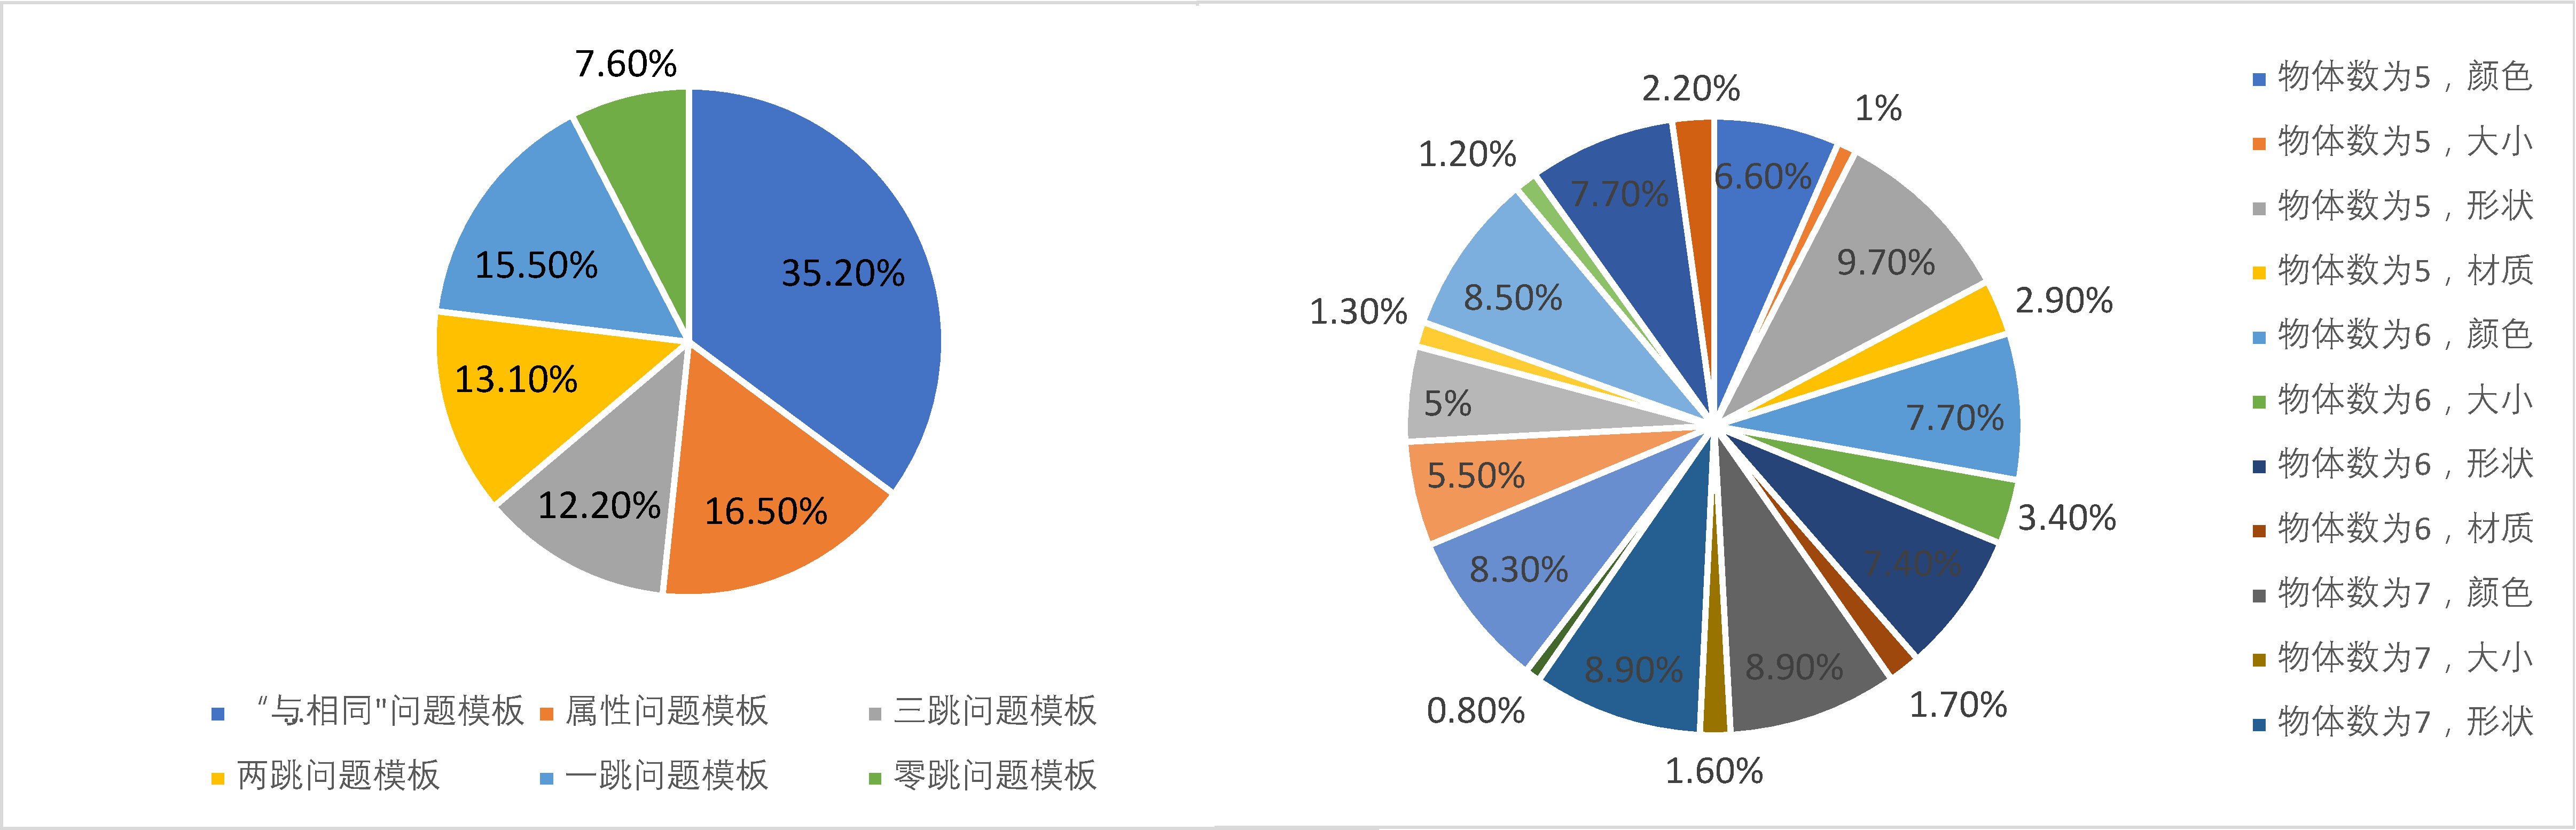
\includegraphics[width=\textwidth]{figures/template_combined-crop.pdf}
    \caption{问题模板统计及问题数量在5到9之间的查询属性分布统计}
    \label{fig:template_statistics}
\end{figure}

问题分布的统计图见图\ref{fig:question_statistics}。从统计图中可得知,有关颜色和形状的问题在SRASP数据集中
占比最高,分别是39\%和37.6\%,关于大小和材质的问题则相对较少,分别只占到了13.1\%和10.3\%。
此外,统计图中也展示了不同类型问题的答案集分布。在生成数据集的过程中尽量实现均衡分布,避免多数问题
指向相同答案集的情况。例如,当问题涉及物体尺寸时,其潜在解可能为\{大、中\}、\{大、小\}、\{小、中\}、\{大\}、\{中\}或\{小\}。
\begin{figure}
    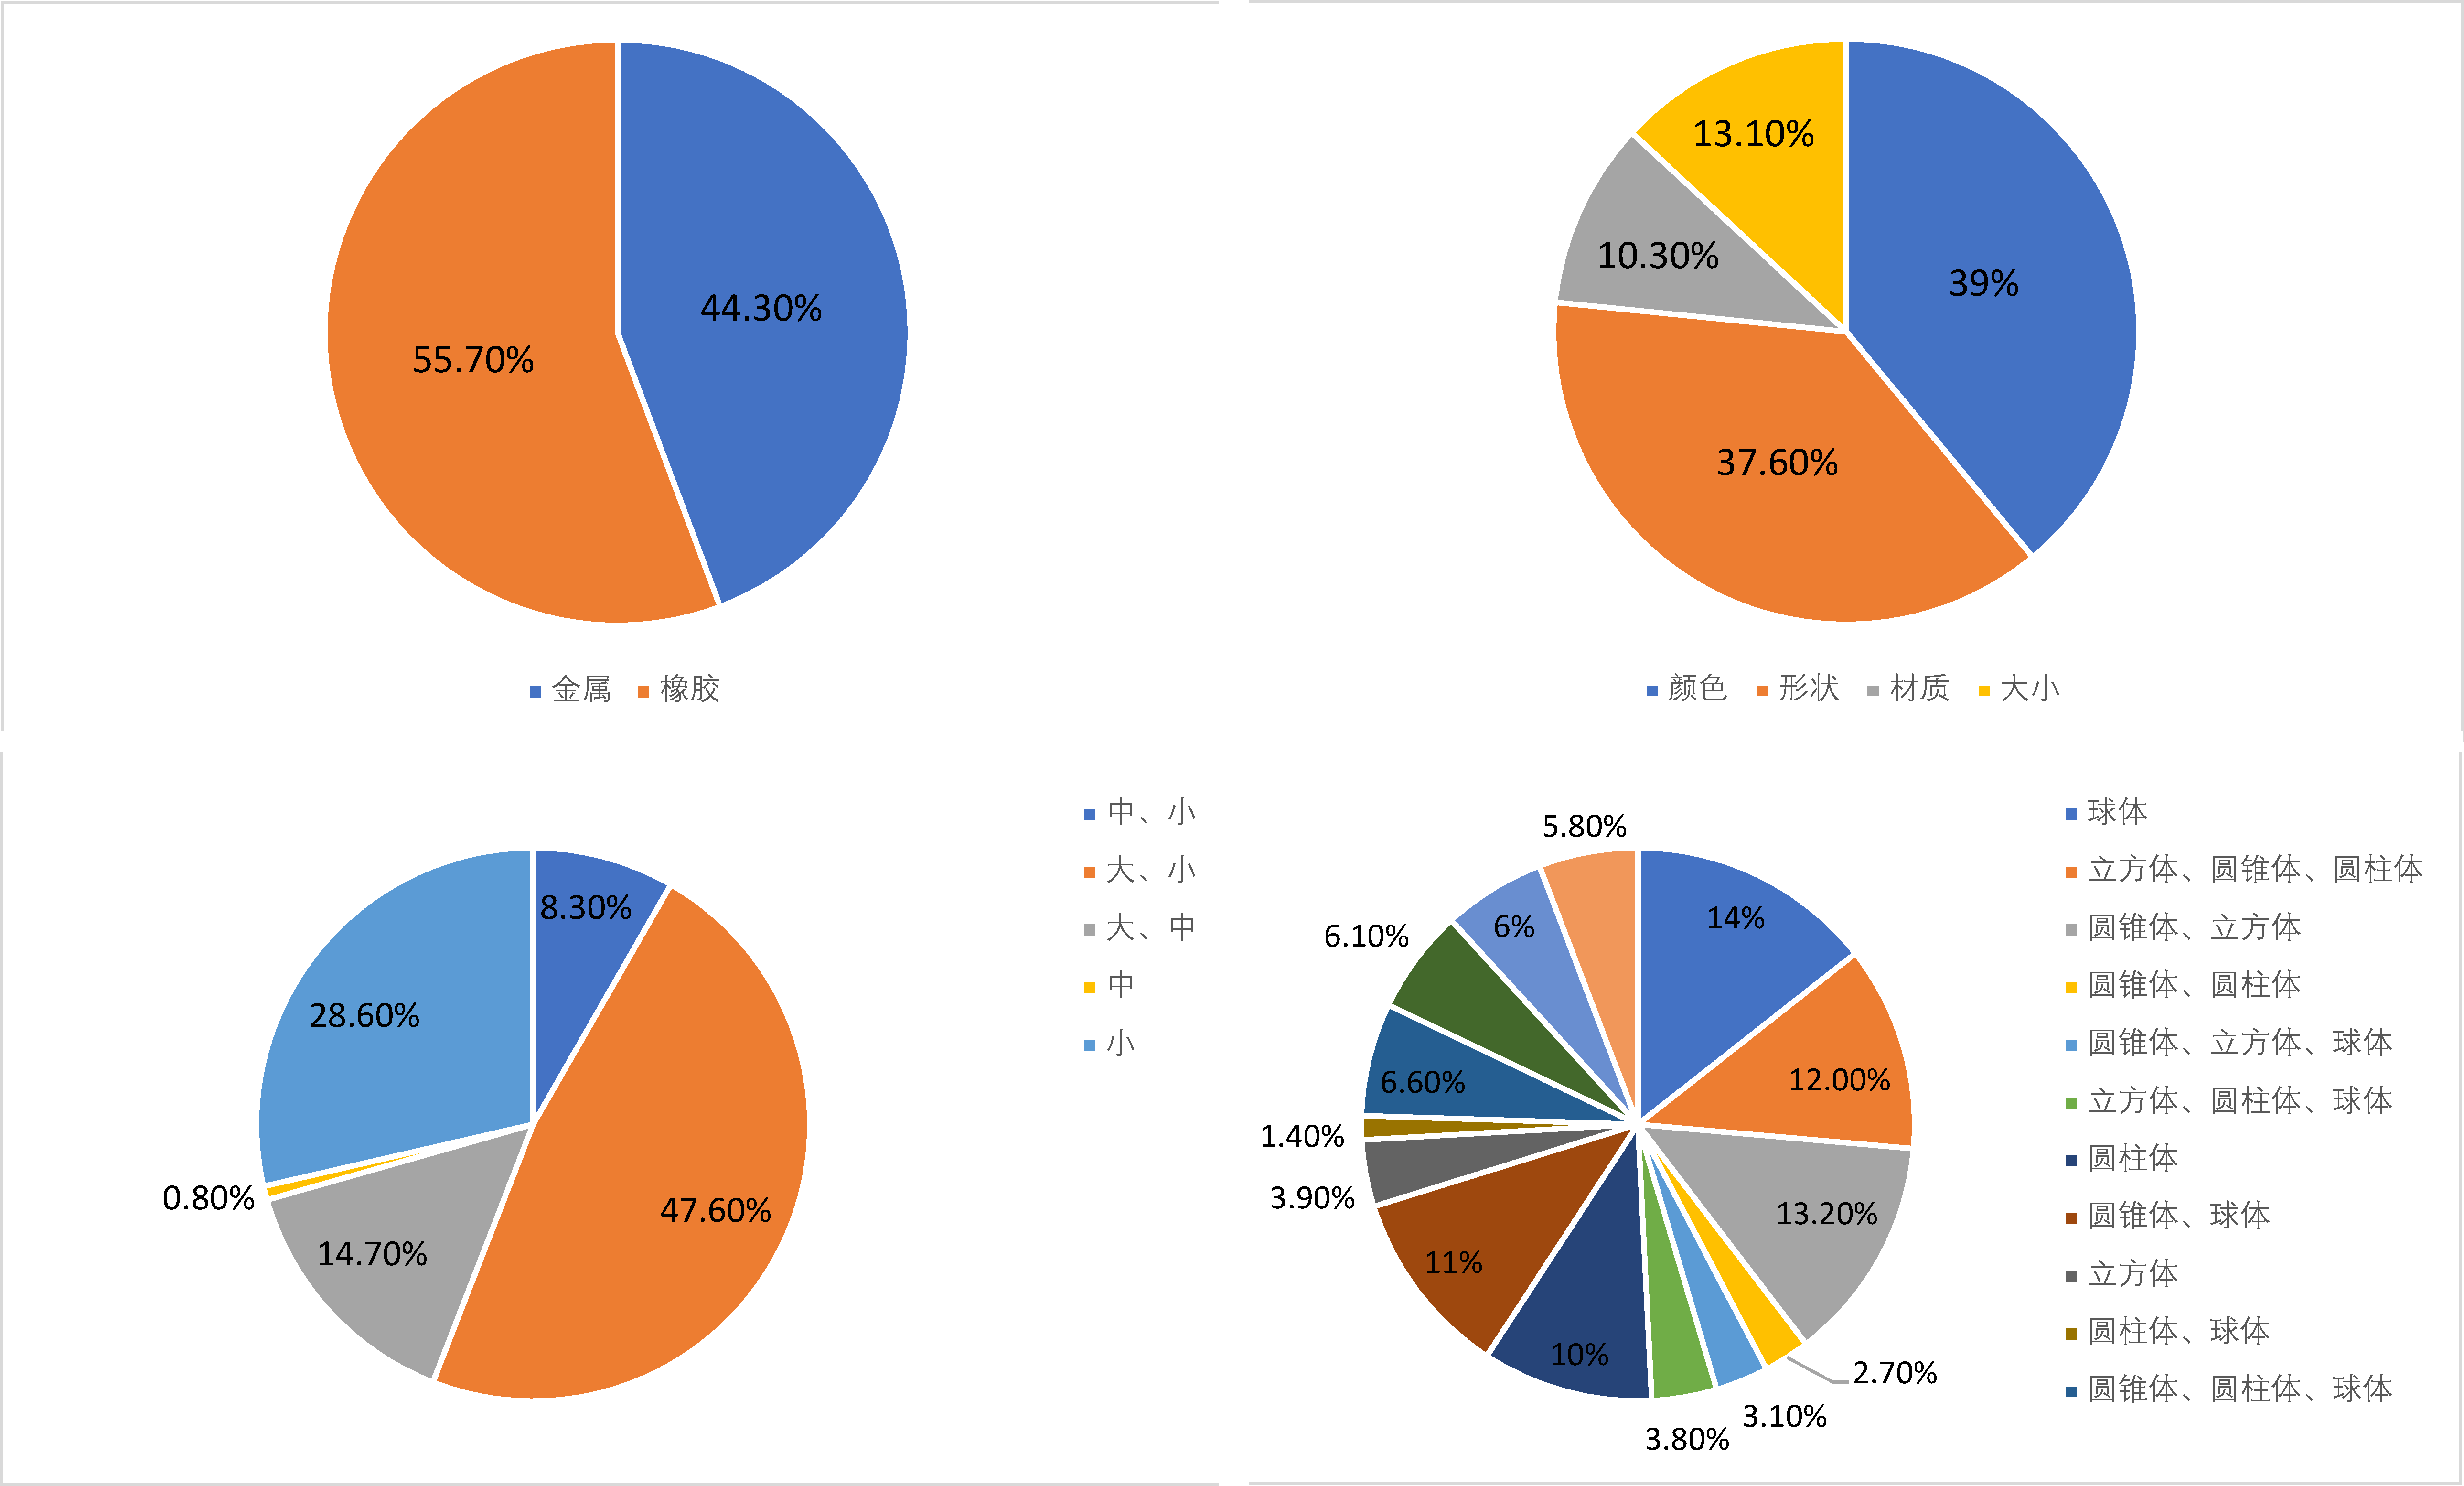
\includegraphics[width=\textwidth]{figures/combined_statistics-crop.pdf}
    \caption{问题分布统计图}
    \label{fig:question_statistics}
\end{figure}

答案的分布统计。
\subsection{质量分析}
\subsubsection{质量保证}
为了保证数据集的质量,采用双盲审核机制,邀请两名评审员各自独立对数据集进行评审,验证每个问题
的答案、推理解答所需步数及问题是否可观察。在评审过程中,如果两名评审员同时判定该问题出现错误,那么
将该问题剔除。双盲评审的结果见表\ref{tab:kappa},其中展示了评审员1和评审员2分别与初始标注的一致性,以及两名评审员
之间的一致性。通过Fleiss's Kappa衡量的评审员间的一致性超过0.8,证明了数据集的可靠性。
\begin{table}[h]
    \centering
    \renewcommand{\arraystretch}{0.8}
    \begin{tabular}{lccc}
    \toprule
     & \makecell{答案是否正确} & \makecell{推理所需步数} & \makecell{问题是否可观察}\\
    \midrule
    初始标注与评审员1 & 81.2 & 84.4 & 89.6 \\
    初始标注与评审员2 & 84.2 & 85.6 & 85.4 \\
    评审员1与评审员2 & 80.1 & 83.8 & 86.9 \\
    \midrule
    平均值 & 81.8 & 84.6 & 87.3 \\
    \bottomrule
    \end{tabular}
    \label{tab:kappa}
    \caption{评审员1、2和初始标注之间的标注者间一致性}
\end{table}
\subsubsection{难度保证}
本文通过记录2位评审员在SRASP数据集上回答问题时的正确率、以及所需检索信息的次数、回答问题所需要的跳数,来对
数据集的难度进行判断,并于其它现有的VQA数据集进行比较。实验结果见表\ref{tab:human_performance},其中明显可以看出,SRASP回答问题所需
的跳数,明显大于现有数据集VQAv2,另外SRASP所需的检索信息的次数也更多一些,这些都证明了回答SRASP数据集
所需的外部知识更多,考虑次数更多,数据集难度更大。另外,人类在本文
构造的SRASP数据集上的准确率最低,进一步侧面印证了本文构造数据集的挑战性。
\begin{table}[h]
    \centering
    \renewcommand{\arraystretch}{0.8}
    \begin{tabular}{lccc}
    \toprule
     & \makecell{回答问题正确率} & \makecell{推理所需跳数} & \makecell{检索信息次数}\\
    \midrule
    SRASP & 81.2 & 84.4 & 89.6 \\
    CLEVR & 84.2 & 85.6 & 85.4 \\
    GQAv2 & 80.1 & 83.8 & 86.9 \\
    \midrule
    平均值 & 81.8 & 84.6 & 87.3 \\
    \bottomrule
    \end{tabular}
    \label{tab:human_performance}
    \caption{人类评审员在不同VQA数据集上回答问题的表现}
\end{table}
\section{本章小结}
本章介绍了SRASP数据集的构造过程,重点描述了如何基于完整场景图生成部分场景图,
并通过 ASP 实例化问题模板以确保问题的多样性和合理性。

首先,本章阐述了对象移除的原则,即如何选择查询对象以及如何保证其属性在问题类型上的均衡性。
随后,详细说明了查询模板的填充策略,包括查询属性的选取、参考对象的确定以及空间关系的合理性,
以确保生成的问题符合实际场景。最后,本章介绍了 ASP 求解器在问题生成过程中的作用,
即利用 ASP 规则对部分场景进行推理,以确定查询属性的可能取值范围,从而生成符合逻辑约束的高质量视觉问答数据。

通过上述方法,SRASP数据集不仅保证了问题的可解释性,还增强了对复杂空间关系的推理能力,
为视觉问答任务提供了更具挑战性的数据支持。